\documentclass[class=report, crop=false, 12pt,a4paper]{standalone}
\usepackage{float}
\usepackage{graphicx}
\usepackage{siunitx}
\usepackage{mathtools}
\usepackage{amsmath}
\usepackage{amssymb}
\usepackage{commath}
\usepackage[a4paper,width=150mm,top=25mm,bottom=25mm]{geometry}
\begin{document}
\section{Understanding poles and zeros}
As defined, the transfer function is a rational function in the complex variable $s = \sigma + j \omega$, that is:
\begin{align}
  G(s) = \frac{b_m s^m + b_{m-1}s^{m-1} + ... + b_1 s + b_0}{a_m s^m + a_{m-1}s^{m-1} + ... + a_1 s + a_0}
\end{align}
It is often convenient to factor the polynomials in the numerator and denominator, and to write the transfer function in terms of those factors:
\begin{align}
  G(s) = \frac{N(s)}{D(s)} = K\frac{(s-z_1)(s-z_2)...(s-z_{m-1})(s-z_m)}{(s-p_1)(s-p_2)...(s-p_{n-1})(s-p_n)}
\end{align}
where the numerator and denominator polynomials, $N(s)$ and $D(s)$, have real coefficients defined by the system's differential equation and $K = \frac{b_m}{a_n}$. Poles and zeros are found by
\begin{align}
  N(s) = 0 \textrm{ and } D(s) = 0 
\end{align}
All of the coefficients of polynomials $N(s)$ and $D(s)$ are real, therefore the poles and zeros must be either purely real, or appear in complex conjugate pairs.
\begin{quote}
  The poles and zeros are properties of the transfer function, and therefore of the differential equation describing the input-output system dynamics. Together with the gain constant, the completely characterise the differential equation, and provide a complete description of the system.
\end{quote}
\subsection{Example}
A linear system is described by the differential equation:
\begin{align}
  \frac{\dif^2 y}{\dif t^2} + 2 \frac{\dif y}{\dif t} + 5y &= 3 \frac{\dif u}{\dif t} + 12 u\\
  \mathcal{L} \left\{ \frac{\dif^2 y}{\dif t^2} + 2 \frac{\dif y}{\dif t} + 5y \right\} &= s^2 Y(s) + 2s Y(s) + 5Y(s)\\
  \mathcal{L} \left\{ 3 \frac{\dif u}{\dif t} + 12 u \right\} &= 3sU(s) + 12U(s)\\
  N(s) = 3s + 12 = 0 \rightarrow z_1 &= -4\\
  D(s) = s^2 + 5s + 5 \rightarrow p_{\frac{1}{2}} &= \frac{-2\pm\sqrt{2^2 - 4\times 5}}{2} &= -1 \pm j2\\
  G(s) = \frac{N(s)}{D(s)} &= 3\frac{s-(-4)}{(s-(-1+j2))(s-(-1-j2))}
\end{align}
\begin{figure}[H]
  \centering
  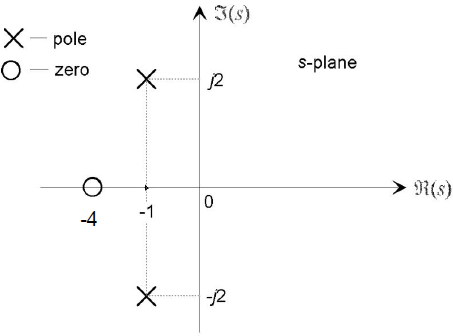
\includegraphics[width = 0.6\textwidth]{../img/diagram67.png}
\end{figure}
\subsection{s-Plane}
We can see how the time domain representation changes as we move around the s-plane. The imaginary axis corresponds to the sinusoidal component, and the real axis corresponds to the exponential.
\begin{figure}[H]
  \centering
  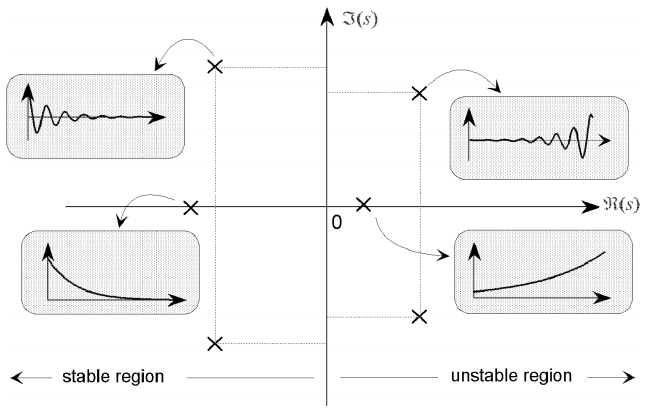
\includegraphics[width = 0.6\textwidth]{../img/diagram68.png}
\end{figure}
\section{Effect of damping ratio on the transfer function of a 2nd order system}
\subsection{2nd order transfer function}
The standard form of second order systems is shown below:
\begin{equation}
  G(s) = \gamma \frac{\omega_n^2}{s^2 + 2\zeta \omega_n s + \omega_n^2}
\end{equation}
where, $\gamma$ is gain, $\omega_n$ is the natural frequency and $\zeta$ is the damping ratio. Luckily the equation is 'standard form' and the time domain result is given directly in Laplace tables:
\begin{align}
  \gamma \frac{\omega_n}{\sqrt{1-\zeta^2}}e^{-\zeta \omega_n t} \sin{\left(\omega_n\sqrt{1-\zeta^2 t}\right)}
\end{align}
But this is only for $\zeta < 1$. Given the damping ratio for a mass spring damper
\begin{align}
  \zeta = \frac{c}{2\sqrt{mk}}, \ \omega_n = \sqrt{\frac{k}{m}}
\end{align}
It is clear the through the choice of $m$, $k$ and $c$ you could create a system with $\zeta \geq 1$.
\subsection{Characteristic equation}
\begin{align}
  G(s) = \gamma \frac{\omega_n^2}{s^2 + 2\zeta \omega_n s + \omega_n^2}
\end{align}
The denominator determines the behaviour of the transfer function, as the numerator is constant. This is known as the \textbf{characteristic equation}. It makes life much simpler if we first try to factor the denominator into first order terms like $(s+a)(s+b)$. So we require the roots of the equation:
\begin{align}
  s^2 + 2\zeta \omega_n s + \omega_n^2
\end{align}
Which can be determined from the quadratic equation:
\begin{align}
  s = -\zeta \omega_n \pm \omega_n \sqrt{\zeta^2 - 1}
\end{align}
Thus it is clear that the roots of the characteristic equations and thus the behaviour of the transfer function is determined by the damping ratio.
\begin{itemize}
  \item Overdamped: $\zeta > 1, \ s = -\zeta \omega_n \pm \omega_n \sqrt{\zeta^2 - 1}$
  \item Critically damped: $\zeta = 1, \ s = -\omega_n$
  \item Underdamped: $0 < \zeta < 1, \ s = -\zeta \omega_n \pm j \omega_n \sqrt{1-\zeta^2}$
  \item Undamped: $\zeta = 0, \ s = \pm j\omega_n$
\end{itemize}
Normally, only the underdamped case is given directly in the Laplace tables, so we need a bit of manipulation to get the others. 
\subsection{Overdamped 2nd order system}
The characteristic equation has two real and negative roots
\begin{gather}
  \zeta > 1\\
  s = - \zeta \omega_n + \omega_n \sqrt{\zeta^2 - 1} = -\alpha\\
  s = - \zeta \omega_n - \omega_n \sqrt{\zeta^2 - 1} = -\beta\\
  \frac{\omega^2}{s^2 + 2\zeta\omega_n s+ \omega_n^2} = \frac{\alpha \beta}{(s+\alpha)(s+\beta)}
\end{gather}
Note: $\alpha \beta = \omega_n^2$. Using partial fractions we can split this into two separate first order systems:
\begin{align}
  \left(\frac{\alpha\beta}{\beta - \alpha}\right) \frac{1}{S + \alpha} + \left(\frac{\alpha\beta}{\alpha - \beta}\right)\frac{1}{S+\beta}
\end{align}
which gives the following in the time domain:
\begin{align}
  x(t) = \alpha \beta \left(\frac{e^{-\alpha t}}{\beta - \alpha} + \frac{e^{-\beta t}}{\alpha - \beta}\right)
\end{align}
\begin{figure}[H]
  \centering
  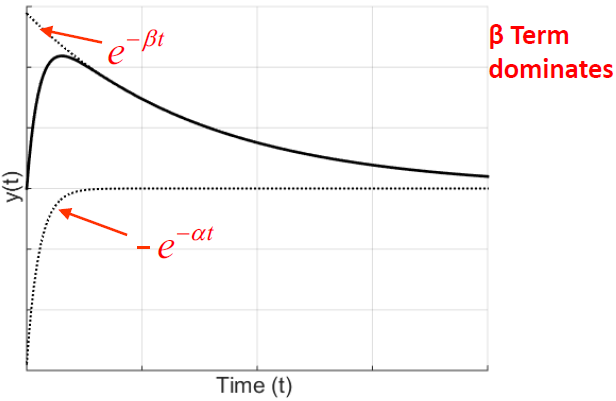
\includegraphics[width = 0.6\textwidth]{../img/diagram69.png}
\end{figure}
There is no sinusoidal term anymore, the response is only a combination of exponential decays, a more complex but similar response to a first order system. 
\subsection{Critically damped 2nd order system}
Special case with a single repeated root:
\begin{gather}
  \zeta = 1\\
  s = -\omega_n\\
  \frac{\omega^2}{s^2 + 2\zeta\omega_n s+ \omega_n^2} = \frac{\omega_n^2}{(s+\omega_n)^2}
\end{gather}
To get the time response, we first take the numerator outside:
\begin{gather}
  L^{-1}\left[ \frac{\omega_n^2}{(s+\omega_n)^2} \right] = \omega_n^2 L^{-1} \left[ \frac{1}{(s+\omega_n)^2} \right]
\end{gather}
We can then use the inverse Laplace rule:
\begin{gather}
  \textrm{if } L^{-1} \left[F(S)\right] = f(t) \textrm{ then } L^{-1} \left[F(s-a)\right] = e^{at} f(t)\\[10pt]
  \omega_n^2 L^{-1} \left[\frac{1}{(s+\omega_n^2)}\right] = \omega_n^2 e^{-\omega_n t} L^{-1} \left[\frac{1}{s^2}\right]
\end{gather}
$\frac{1}{s^2}$ is the standard form of a ramp, or more generally from the Laplace tables:
\begin{align}
  L^{-1}\left[\frac{n!}{s^{n+1}}\right] = t^n
\end{align}
\begin{figure}[H]
  \centering
  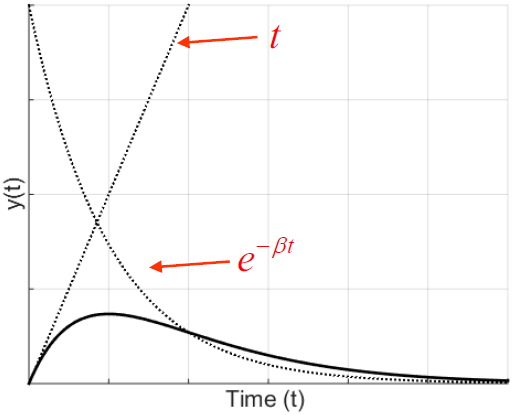
\includegraphics[width = 0.6\textwidth]{../img/diagram70.png}
\end{figure}
The result is an exponential decay, multiplied by a ramp $= \omega_n^2 e^{-\omega_n t} t$.
\subsection{Undamped 2nd order system}
Another special case with two imaginary roots:
\begin{gather}
  \zeta = 0\\
  s = \pm j \omega_n\\
  \frac{\omega^2}{s^2 + 2\zeta\omega_n s+ \omega_n^2} = \frac{\omega_n^2}{s^2 + \omega_n^2}
\end{gather}
Which, using the standard form for an oscillator is:
\begin{equation}
  \omega_n L^{-1} \left[ \frac{\omega_n}{s^2 + \omega_n^2} \right] = \omega_n \sin{(\omega_n t)}
\end{equation}
\begin{figure}[H]
  \centering
  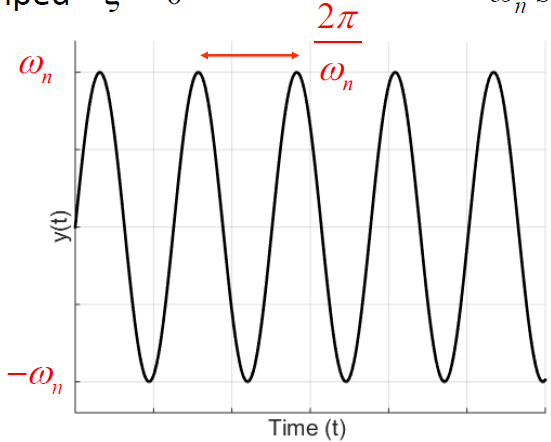
\includegraphics[width = 0.6\textwidth]{../img/diagram71.png}
\end{figure}
So the response is now just a sinusoid, with no exponential components.
\section{Applying a step input to 2nd order systems - damping}
Previously we saw for a step of $A$ the output can be calculated from
\begin{gather}
  Y(s) = \frac{A}{s} G(s)\\
  Y(s) = \frac{1}{s} \cdot \frac{\omega_n^2}{s^2 + 2\zeta \omega_n s \omega_n^2}
\end{gather}
All of the following can be found through partial fraction decomposition and the standard Laplace tables.
\subsection{Overdamped step input response of 2nd order systems}
\begin{gather}
  \zeta > 1\\
  y(t) = \left(1 = \frac{\beta e^{-\alpha t}}{\alpha - \beta} - \frac{\alpha e^{-\beta t}}{\alpha - \beta}\right)
\end{gather}
\begin{figure}[H]
  \centering
  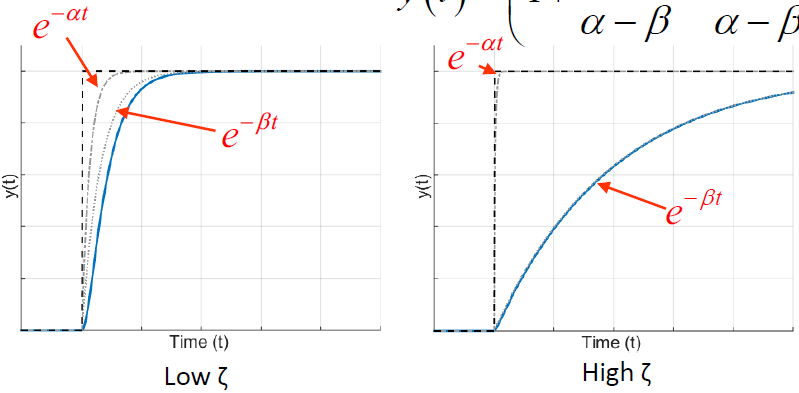
\includegraphics[width = 0.8\textwidth]{../img/diagram72.png}
\end{figure}
The slowest rise from the $\beta$ exponential dominates, as $\zeta$ increases the $\alpha$ term becomes negligible, and system becomes first order. 
\subsection{Critically damped step input response of 2nd order systems}
\begin{gather}
  \zeta = 1\\
  y(t) = \left(1 - e^{-\omega_n t} - \omega_n e ^{-\omega_n t} t\right)
\end{gather}
\begin{figure}[H]
  \centering
  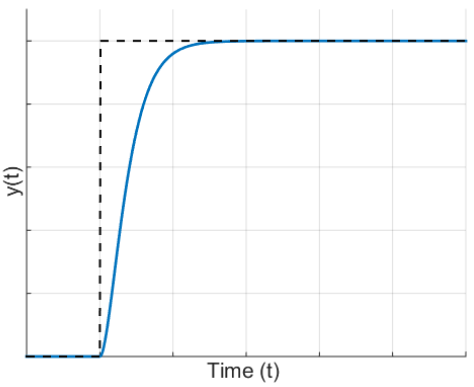
\includegraphics[width = 0.6\textwidth]{../img/diagram73.png}
\end{figure}
Fastest possible rise without oscillating.
\subsection{Underdamped step input response of 2nd order systems}
\begin{gather}
  0 < \zeta < 1 \\
  y(t) = 1 - \frac{1}{\sqrt{1 - \zeta^2}}e^{-\zeta \omega_n t} \sin{\left(\omega_n \sqrt{1-\zeta^2 t} + \arccos{\zeta}\right)}
\end{gather}
\begin{figure}[H]
  \centering
  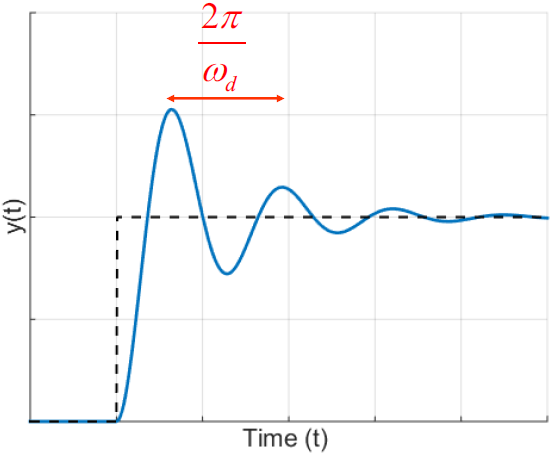
\includegraphics[width = 0.6\textwidth]{../img/diagram74.png}
\end{figure}
It is sometimes written in terms of the damped natural frequency:
\begin{gather}
  \omega_d = \omega_n \sqrt{1-\zeta^2}\\
  y(t) = 1 - \frac{1}{\sqrt{1-\zeta^2}} e^{-\zeta \omega_n t} \sin{\left(\omega_d t + \arccos{\zeta}\right)}
\end{gather}
\subsection{Undamped step input response of 2nd order systems}
\begin{align}
  \zeta = 0 \\
  y(t) = \left(1 - \cos{(\omega_n t)}\right)
\end{align}
As damping ratio reaches zero, the oscillations no longer decay
\begin{equation}
  \omega_d = \omega_n \sqrt{1 - 0} = \omega_n
\end{equation}
So oscillations are at natural frequency with pi phase shift.
\begin{figure}[H]
  \centering
  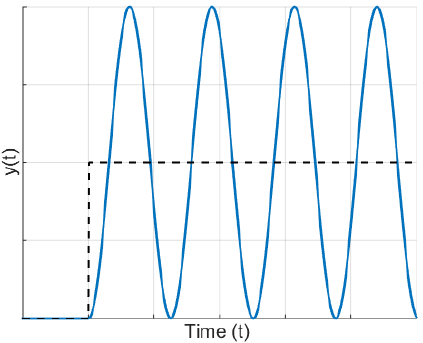
\includegraphics[width = 0.6\textwidth]{../img/diagram75.png}
\end{figure}
\section{Underdamped step input responses}
\subsection{Performance Criteria}
Rise time $t_r$ is the time to reach steady state value (for first time). Peak time $t_p$ is the time to initial overshoot.
\begin{figure}[H]
  \centering
  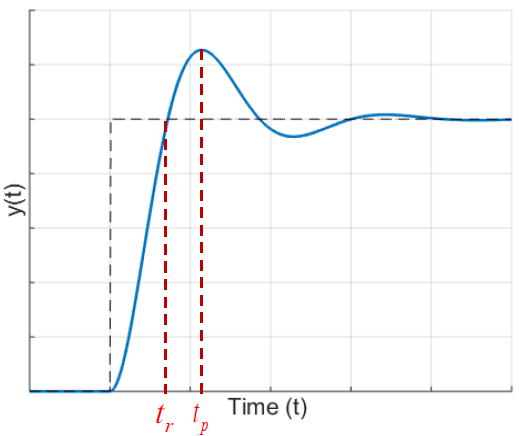
\includegraphics[width = 0.6\textwidth]{../img/diagram76.png}
\end{figure}
Peak overshoot - value of overshoot above steady state: $ y(t_p) - y_{ss} = A$. Settling time $t_s$. Time for response to reach and maintain a certain ratio of the steady state value. Commonly $\pm 5\%$ or $\pm 2\%$
\begin{figure}[H]
  \centering
  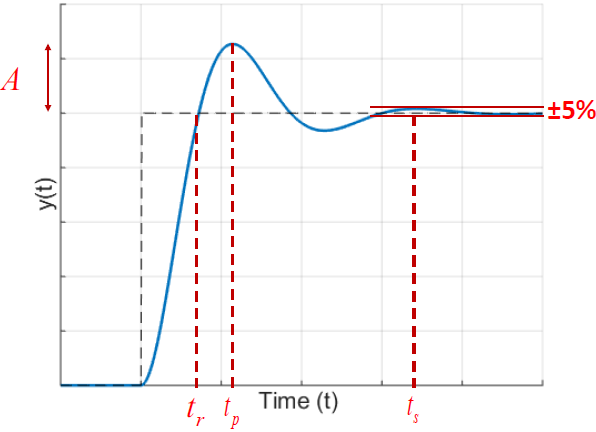
\includegraphics[width = 0.6\textwidth]{../img/diagram77.png}
\end{figure}
These criteria can be read from the graph, but having equations for them allows for a system parameters $\zeta$ and $\omega_n$ to be estimated. It is also useful for quantifying the effect of $\zeta$ on the response. Rise time can be found by setting the response $y$ to 1 and then rearranging:
\begin{equation}
  t_r = \frac{1}{\omega_d} \left( \pi - \arctan{\left( \frac{\sqrt{1-\zeta^2}}{\zeta} \right)} \right)\\
  \omega_d = \omega_n \sqrt{1-\zeta^2}
\end{equation}
So a higher damping ratio gives a slower response, but lower damping ratios give a more oscillatory response. Also, that for \textbf{overdamped} systems where $\zeta > 1$, the rise time is infinite. The peak time occurs at half a period of oscillation, or can be found from finding first minima by setting derivative to zero:
\begin{equation}
  t_p = \frac{\pi}{\omega_n\sqrt{1 - \zeta^2}} = \frac{\pi}{\omega_d}
\end{equation}
\subsubsection{Peak overshoot}
\begin{gather}
  1 + A = 1 - \frac{1}{\sqrt{1 - \zeta^2}} e^{\frac{-\zeta \pi}{\sqrt{1-\zeta^2}}}\sin{\left(\pi + \arccos{\zeta}\right)}\\[10pt]
  A = \frac{\sqrt{1-\zeta^2}}{\sqrt{1-\zeta^2}} e^{\frac{-\zeta \pi}{\sqrt{1-\zeta^2}}} = e^{\frac{-\zeta \pi}{\sqrt{1-\zeta^2}}}
\end{gather}
Often, this is given as a percentage:
\begin{equation}
  A = 100 e^{\frac{-\zeta \pi}{\sqrt{1-\zeta^2}}}
\end{equation}
This can be rearranged to find the required damping ratio for a required overshoot:
\begin{gather}
  \zeta = \sqrt{\frac{\left(\ln{\frac{A}{100}}\right)^2}{\pi^2 + \left(\ln{\frac{A}{100}}\right)^2}}\\
  \frac{A}{100} \rightarrow 0\\
  \zeta \rightarrow 1
\end{gather}
\subsubsection{Settling time}
The envelope of the oscillation is described by the decaying exponential term, so to find the settling time, we can just consider this term alone.
\begin{figure}[H]
  \centering
  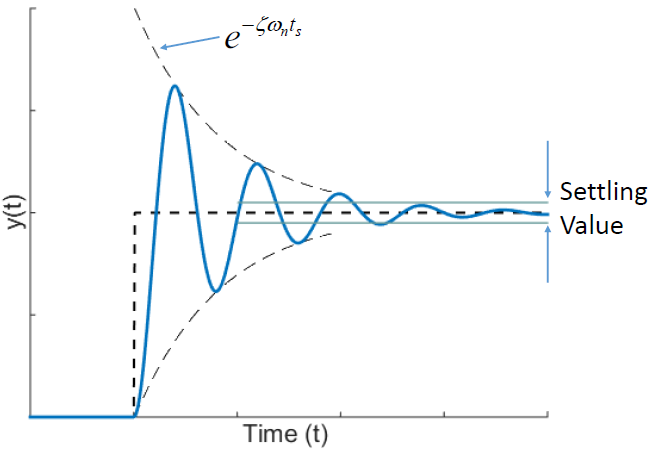
\includegraphics[width = 0.6\textwidth]{../img/diagram78.png}
\end{figure}
For example, the common target is 5\%:
\begin{gather}
  e^{-\zeta \omega_n t_s} = 0.05\\
  -\zeta \omega_n t_s = \ln{0.05} = -3\\
  t_s (5\%) = \frac{3}{\zeta \omega_n}
\end{gather}
Or similarly:
\begin{equation}
  t_s (2\%) = \frac{4}{\zeta \omega_n}
\end{equation}
So settling time increases with a \textbf{decreasing} damping ratio, for underdamped systems only.
\section{Ramp input function responses}
\subsection{Applying inputs}
Previously, we saw for a step of $A$ the output can be calculated from:
\begin{gather}
  Y(s) = \frac{A}{s^2} G(s)\\
  Y(s) = \frac{1}{s^2} \frac{\omega_n^2}{s^2 + 2\zeta \omega_n s + \omega_n^2}
\end{gather}
All the following can be found through partial fraction decomposition and the standard Laplace tables (and loads more manipulation!). All these expressions are pretty complicated, but the important thing is to understand how the response changes with damping ratio, which follows a similar trend to the step response. 
\subsection{Undamped response}
$\zeta = 0$: undamped - sustained oscillations around ramp input $y = t$.
\begin{equation}
  y(t) = \left(t - \frac{\sin(\omega_n t)}{\omega_n}\right)
\end{equation}
\begin{figure}[H]
  \centering
  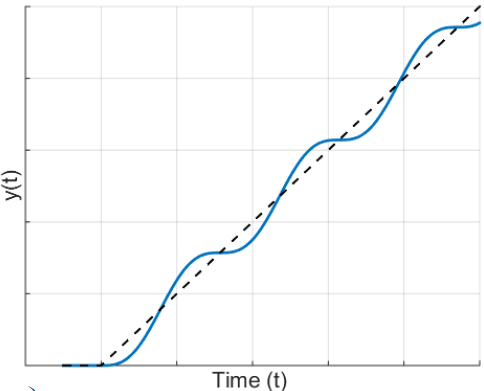
\includegraphics[width = 0.6\textwidth]{../img/diagram79.png}
\end{figure}
\subsection{Underdamped response}
$\zeta < 1$: underdamped - exponential decaying oscillatory response around delayed ramp function.
\begin{multline}
  y(t) = \frac{1}{\omega_n} \left( \omega_n t - 2\zeta + e^{-\zeta \omega_n t} \left( 2\zeta \cos\left( \omega_n t\sqrt{1 - \zeta^2} \right) \right. \right. \\ 
  \left. \left. - \frac{1}{\sqrt{1-\zeta^2}} \left( 1 - 2\zeta^2 \right) \sin \left( \omega_n t\sqrt{1-\zeta^2} \right) \right) \right)
\end{multline}
\begin{figure}[H]
  \centering
  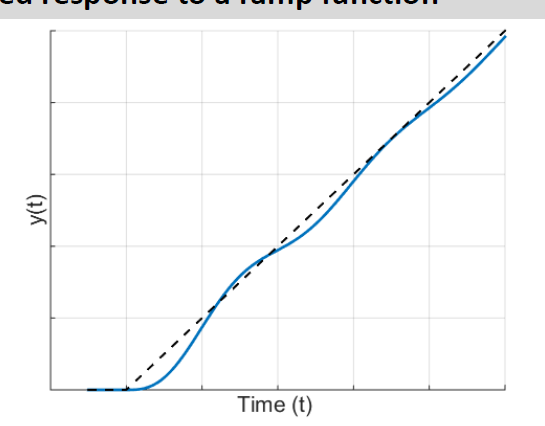
\includegraphics[width = 0.6\textwidth]{../img/diagram80.png}
\end{figure}
\subsection{Critically damped response}
$\zeta = 1$: Critically damped - fastest response with no overshoot, still lagging input.
\begin{equation}
  y(t) = \frac{1}{\omega_n} \left(\omega_n t - 2 + \left(2 + \omega_n t\right)e^{-\omega_n t}\right)
\end{equation}
\begin{figure}[H]
  \centering
  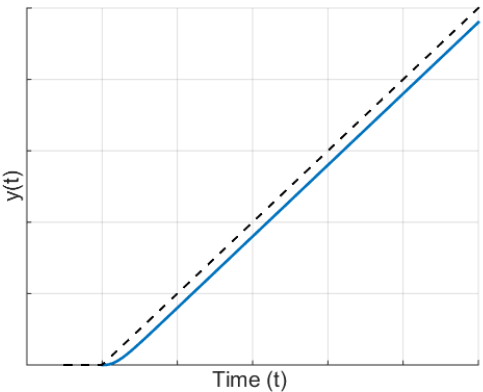
\includegraphics[width = 0.6\textwidth]{../img/diagram81.png}
\end{figure}
\subsection{Overdamped response}
$\zeta > 1$: overdamped - cannot overshoot, lag increases.
\begin{equation}
  y(t) = \left(t -\frac{2\zeta}{\omega_n} + \frac{\beta e^{-\alpha t}}{\alpha - \beta} - \frac{\alpha e^{-\beta t}}{\alpha - \beta} \right)
\end{equation}
\begin{figure}[H]
  \centering
  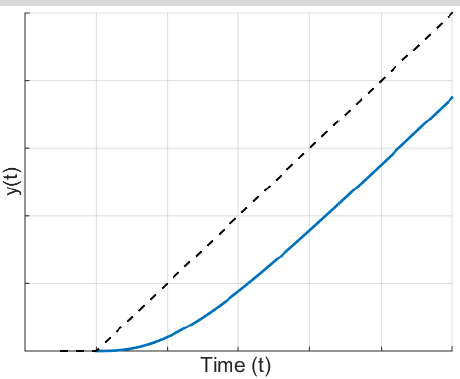
\includegraphics[width = 0.6\textwidth]{../img/diagram82.png}
\end{figure}
\subsection{Summary}
Much more complicated response! but follows the same pattern as with the step response with changing damping ratio. The most important thing to notice here, is that the system does not match desired value - there is still a lag:
\begin{equation}
  y(t) = t - \frac{2\zeta}{\omega_n}
\end{equation}
So a low damping ratio is needed to closely match the input value, but this comes at the expense of overshoot and settling time.
\section{Transfer function - unity feedback system}
Recall the block diagram for a closed loop feedback system, in this case with 'unity' feedback - i.e. the error signal is passed directly to the summation junction:
\begin{figure}[H]
  \centering
  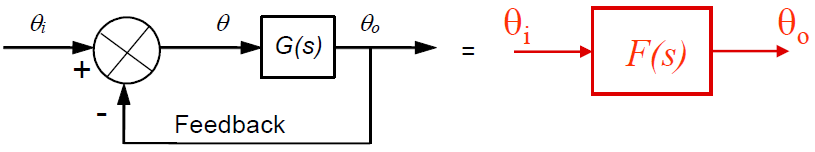
\includegraphics[width = 0.9\textwidth]{../img/diagram83.png}
\end{figure}
$G(s)$ is referred to as the \textbf{forward loop transfer function}, i.e. the combined transfer function of all the amplifiers controller, plant, systems in the feedforward path. In the case of unity feedback, it is also the \textbf{open loop transfer function}. We can find the overall transfer function $F(s)$ or \textbf{closed loop transfer function} through a bit of manipulation:
\begin{gather}
  \theta = \theta_i - \theta_0\\
  G(s)\theta = \theta_0\\
  \theta_0 = G(s) (\theta_i - \theta_0)\\
  \frac{\theta_0}{\theta_i} = F(s) = \frac{G(s)}{1 + G(s)}
\end{gather}
Or more generally for a non unity gain system:
\begin{figure}[H]
  \centering
  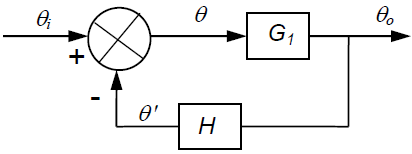
\includegraphics[width = 0.6\textwidth]{../img/diagram84.png}
\end{figure}
\begin{equation}
  F_1 = \frac{\theta_0}{\theta_i} = \frac{G_1}{1 + G_1 H}
\end{equation}
Lets take an example to show how this transfer function can relate to the systems we have studied so far.
\section{Summary}
\begin{figure}[H]
  \centering
  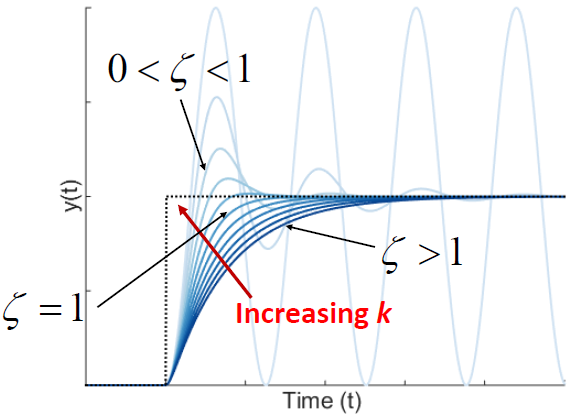
\includegraphics[width = 0.6\textwidth]{../img/diagram85.png}
\end{figure}
The overdamped ($\zeta > 1$) and critically damped ($\zeta = 1$) responses are seldom desirable for control systems due to their long settling time. $\zeta = 0.7$ gives a fast response without excessive overshoot or oscillations.
\begin{figure}[H]
  \centering
  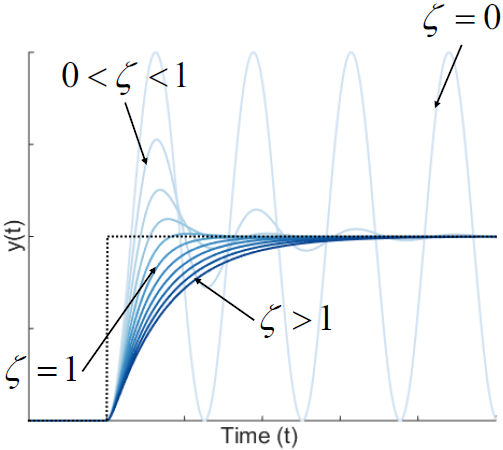
\includegraphics[width = 0.6\textwidth]{../img/diagram86.png}
\end{figure}
The response of second order systems is much more complicated than that of a first order system, with considerably different responses arising from changes in damping ratio.
\begin{figure}[H]
  \centering
  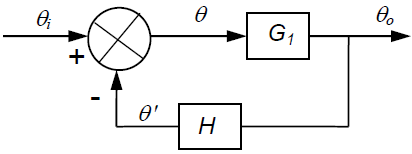
\includegraphics[width = 0.6\textwidth]{../img/diagram84.png}
\end{figure}
Negative feedback systems have a transfer function of the form:
\begin{equation}
  F_1 = \frac{\theta_0}{\theta_i} = \frac{G_1}{1 + G_1 H}
\end{equation}
Which for a remote position servo is equal to:
\begin{equation}
  F(s) = \frac{\Theta_0 (s)}{\Theta_i (s)} = \frac{\frac{k}{I}}{s^2 + \frac{f}{I}s + \frac{k}{I}}
\end{equation}
Where $\omega_n = \sqrt{\frac{k}{I}}$ and $\zeta = \frac{f}{2\sqrt{kI}}$. The gain determines the damping ratio, and this the characteristics of the response of the system.
\end{document}